%% Copernicus Publications Manuscript Preparation Template for LaTeX Submissions
%% ---------------------------------
%% This template should be used for copernicus.cls
%% The class file and some style files are bundled in the Copernicus Latex Package, which can be downloaded from the different journal webpages.
%% For further assistance please contact Copernicus Publications at: production@copernicus.org
%% https://publications.copernicus.org/for_authors/manuscript_preparation.html


%% Please use the following documentclass and journal abbreviations for discussion papers and final revised papers.

%% 2-column papers and discussion papers
\documentclass[nhess, manuscript]{copernicus}



%% Journal abbreviations (please use the same for discussion papers and final revised papers)


% Advances in Geosciences (adgeo)
% Advances in Radio Science (ars)
% Advances in Science and Research (asr)
% Advances in Statistical Climatology, Meteorology and Oceanography (ascmo)
% Annales Geophysicae (angeo)
% Archives Animal Breeding (aab)
% ASTRA Proceedings (ap)
% Atmospheric Chemistry and Physics (acp)
% Atmospheric Measurement Techniques (amt)
% Biogeosciences (bg)
% Climate of the Past (cp)
% DEUQUA Special Publications (deuquasp)
% Drinking Water Engineering and Science (dwes)
% Earth Surface Dynamics (esurf)
% Earth System Dynamics (esd)
% Earth System Science Data (essd)
% E&G Quaternary Science Journal (egqsj)
% European Journal of Mineralogy (ejm)
% Fossil Record (fr)
% Geochronology (gchron)
% Geographica Helvetica (gh)
% Geoscience Communication (gc)
% Geoscientific Instrumentation, Methods and Data Systems (gi)
% Geoscientific Model Development (gmd)
% History of Geo- and Space Sciences (hgss)
% Hydrology and Earth System Sciences (hess)
% Journal of Micropalaeontology (jm)
% Journal of Sensors and Sensor Systems (jsss)
% Magnetic Resonance (mr)
% Mechanical Sciences (ms)
% Natural Hazards and Earth System Sciences (nhess)
% Nonlinear Processes in Geophysics (npg)
% Ocean Science (os)
% Primate Biology (pb)
% Proceedings of the International Association of Hydrological Sciences (piahs)
% Scientific Drilling (sd)
% SOIL (soil)
% Solid Earth (se)
% The Cryosphere (tc)
% Weather and Climate Dynamics (wcd)
% Web Ecology (we)
% Wind Energy Science (wes)


%% \usepackage commands included in the copernicus.cls:
%\usepackage[german, english]{babel}
%\usepackage{tabularx}
%\usepackage{cancel}
%\usepackage{multirow}
%\usepackage{supertabular}
%\usepackage{algorithmic}
%\usepackage{algorithm}
%\usepackage{amsthm}
%\usepackage{float}
%\usepackage{subfig}
%\usepackage{rotating}
\usepackage{siunitx}
\DeclareSIUnit\year{yr}



\begin{document}

\title{Leveraging time series analysis of radar coherence and NDVI ratios to characterize pre-failure activity of the Mud Creek landslide, California}


% \Author[affil]{given_name}{surname}

\Author[1]{Mylène}{Jacquemart}
\Author[1]{Kristy}{Tiampo}
%\Author[]{}{}

\affil[1]{Cooperative Institute for Research in Environmental Sciences (CIRES), University of Colorado, Boulder}
%\affil[]{ADDRESS}

%% The [] brackets identify the author with the corresponding affiliation. 1, 2, 3, etc. should be inserted.

%% If an author is deceased, please mark the respective author name(s) with a dagger, e.g. "\Author[2,$\dag$]{Anton}{Aman}", and add a further "\affil[$\dag$]{deceased, 1 July 2019}".

%% If authors contributed equally, please mark the respective author names with an asterisk, e.g. "\Author[2,*]{Anton}{Aman}" and "\Author[3,*]{Bradley}{Bman}" and add a further affiliation: "\affil[*]{These authors contributed equally to this work.}".


\correspondence{Mylène Jacquemart (mylene.jacquemart@colorado.edu)}

\runningtitle{TEXT}

\runningauthor{TEXT}





\received{}
\pubdiscuss{} %% only important for two-stage journals
\revised{}
\accepted{}
\published{}

%% These dates will be inserted by Copernicus Publications during the typesetting process.


\firstpage{1}

\maketitle



\begin{abstract}
Assessing landslide activity at large scales has historically been a challenging problem. Here, we present a different approach on radar coherence and normalized difference vegetation index (NDVI) analyses - metrics that are typically used to map landslides post-failure - and leverage a time series analysis to characterize the pre-failure activity of the Mud Creek landslide in California. Our method computes the ratio of mean interferometric coherence or NDVI on the unstable slope relative to that of the surrounding hillslope. This approach has the advantage that it eliminates the negative impacts of long temporal baselines that can interfere with the analysis of interferometric synthetic aperture (InSAR) data, as well as interferences from atmospheric and environmental factors. We show that the coherence ratio of the Mud Creek landslide dropped by 50\% when the slide began to accelerate five months prior to its catastrophic failure in 2017. Coincidentally, the NDVI ratio began a near-linear decline. A similar behavior is visible during an earlier acceleration of the landslide in 2016. This suggests that radar coherence and NDVI ratios may be useful for assessing landslide activity. Our study demonstrates that data from the ascending track provides the more reliable coherence ratios, despite being poorly suited to measure the slope's precursory deformation. Combined, these insights suggest that this type of analysis may complement traditional InSAR analysis in useful ways and provide an opportunity to assess landslide activity at regional scales.  
\end{abstract}


\copyrightstatement{TEXT}


\introduction  %% \introduction[modified heading if necessary]
Landslides are among the most destructive and costly natural hazards and their occurrence and impacts remain difficult to predict. The numerous triggering processes and controls on landslide size, runout distance or time of failure make it hard to assess the risks and potential impacts for even just a single hillslope. Carrying out such an assessment at the regional level is a comparatively harder challenge. Yet assessing landslide activity over larger regions can be crucial to effective hazard management \citep{vanwesten2006}. Remote sensing techniques using both optical imagery and satellite radar data have long been recognized as useful tools to carry such regional scale assessments \citep{mantovani1996, rosin2005}. However, while many of these efforts are focused on mapping landslides after they have occurred, assessing the activity of landslides is a harder problem.
The most reliable and common approaches for assessing landslide activity and potential for failure rely on measurements of slope displacements and derivatives thereof \citep{intrieri2019}. For individual, known instabilities, this is most commonly achieved through on-site monitoring systems using GPS, crack meters, image analysis, automated theodolite measurements or ground based radar and lidar measurements \citep[e.g.,][]{gili2000, chelli2006, kos2016, loew2016}. Monitoring landslide activity has also been achieved with aerial images and high resolution satellite images, though the focus thereof lies more on individual instabilities than on entire regions \citep[e.g.,][]{hervas2003}. Recently, interferometric synthetic aperture radar (InSAR) techniques have gained popularity for assessing landslide activity because they provided the opportunity to measure slope displacements over large areas. Despite this advantage, Norway is presently the only county systematically leveraging radar interferometry for a country-wide monitoring effort \citep{lauknes2010, dehls2014}.   \par 

Generating robust displacement time series from InSAR, despite its all-weather and day-and-night capability, is not without challenges. Due to its oblique viewing geometry, radar can be rendered useless in areas of steep topography due to the effects of shadowing and layover (the compression of a large area into only few image pixels) \citep{wasowski2014, lillesand2015}. In areas not affected by these geometric artefacts, the maximum detectable deformation gradient is equal to half the wavelength per image pixel ($\frac{\lambda}{2}$; \cite{massonnet1998}. Because radar instruments only measure the component of motion in line of sight, the the measurable deformation is strongly controlled by the viewing geometry \citep{massonnet1998}. Further difficulties include the relative nature of radar measurements, making it necessary to know or assume a stable location where there is no deformation, as well as the fact that radar measurements are 2$\pi$ wrapped \citep{wasowski2014, massonnet1998}. The wrapped nature of the data requires that radar measurements are unwrapped to derive the actual displacement in meters rather than radians \citep{massonnet1998, chen2002}. This process is computationally expensive and phase unwrapping errors can mask the full displacement \citep{wasowski2014}. Additionally, in order to reliably measure ground displacements, the wave scattering properties of ground targets must remain unchanged between two radar measurements \citep{massonnet1998, zebker1992}.  \par 

This similarity between two radar images is expressed in the radar coherence metric, which is the primary indicator of radar data quality and can be impacted by several different factors. Generally speaking, a reduction in radar coherence indicates that either the scattering properties of the target have changed (temporal decorrelation) or that the imaging geometry has shifted substantially (spatial decorrelation; \cite{zebker1992, rosen2000}). Instrument noise (signal-to-noise ratio) can also be a cause of coherence loss (thermal decorrelation), but is typically small in modern systems \citep{zebker1992}. When radar images are re-acquired from the same position, spatial decorrelation is minimized and coherence changes are predominantly temporal in nature. This can be exploited for detecting changes such as soil moisture variations, ground deformation, and ground cover or land use change such as those caused by vegetation cycles, agricultural practices, or damage from natural hazards \citep[e.g.][]{burrows2019, fielding2005, yun2015, musa2015}. \par 

These variations in coherence can also be efficiently exploited for landslide mapping. When large numbers of landslides are triggered by earthquakes or tropical storms, fast and precise landslide mapping is key for organizing effective rescue efforts. The increased availability of SAR data (e.g., freely available Sentinel-1 imagery from the European Space Agency ESA) has led to significant developments in this regard. Coherence-based landslide mapping has been achieved using absolute coherence thresholds, differences between pre-event and co-event or co-event and post-event coherence maps, as well as coherence time series analyses \citep{burrows2019, yun2015, ohki2020, jung2020}. \par 

Optical images have also been used to map landslides, but are significantly limited in their utility due to cloud cover, shadows and darkness. If high-resolution optical images are available, landslides are frequently mapped by hand, a process that is tedious and time consuming \citep[e.g.][]{roback2018}. To speed up the production of such landslide inventories, automated and semi-automated procedures have been developed \citep{guzzetti2012, fiorucci2019, behling2014, behling2014a, mondini2011}. Many of the (semi-)automated methods make use of the damage that landslides cause to plants, which can be detected in multispectral optical images using vegetation indices like the Normalized Difference Vegetation Index (NDVI; \cite{tucker1979, Rosenthal1985}). Either of these techniques can be severely limited if good ground visibility is not provided, a situation that is particularly common after rainfall-induced landslide events. \par

Both radar coherence and NDVI based approaches described above offer the possibility to effectively map landslides over large regions, but so far they have been applied purely after landslide events. Here, for the first time, we used time series analysis of radar coherence and NDVI to investigate the behavior of the Mud Creek landslide in California \textit{before} its catastrophic failure in May 2017. We generated the time series by calculating the ratios between the mean coherence (or mean NDVI) on the slide and that of the surrounding hillslope and then compared these time series to precursory deformation computed by ourselves and \cite{handwerger2019}. Finally, we assessed the usefulness of these indicators to assess landslide stability and discuss the possibility of using them at regional scales with and without prior knowledge of a landslide location. 

In the following, we describe the general setting of the Mud Creek landslide (Section \ref{sec:study_site}) and the methodology, data selection and methodological assumptions (Section \ref{sec:methods}). In section \ref{sec:results} we present our findings, and in section \ref{sec:discussion} we discuss these in the context of landslide monitoring and lay out the need and opportunities for future research. 

%InSAR has also been applied to detect precursory acceleration of the 20 May 2017 Mud Creek landslide in California. \cite{Handwerger2019} showed that the seasonal accelerations of the Mud Creek landslide could be tracked throughout the period for which radar data is available, and that a larger speed-up occurred in the months prior to the failure. An acceleration of a landslide body is considered the best indicator for a future failure; however, determining how much acceleration is indicative of impending failure remains unknown. As with the Mud Creek landslide, unstable slopes frequently accelerate seasonally, or in response to temperature changes or precipitation, without failing catastrophically \citep{iverson2000, Segui2020, handwerger2013}. \par 





\section{Study site}
\label{sec:study_site}
The Santa Lucia Mountains rise abruptly from the Pacific Ocean on California's Big Sur Coast, a geologically complex region about 150 miles south of San Francisco (Fig. \ref{fig:overview}). Formed in a transpression zone of the San Gregorio-Hosgri Fault System known as the Big Sur Bend, the crest of this rugged, high-relief mountain range rises to over 1700 m asl and is never more than 18\,km from the coast \citep{Johnson2018}. Geologically, Miocene marine sediments, Mesozoic to Precambrian granitic and metamorphic rocks, as well as Cretaceous-Jurassic marine sedimentary and metasedimentary rocks make up the Santa Lucia Mountains \citep{graham1978}. The Franciscan Mélange that dominates the geology near Mud Creek consists of mesozoic graywacke sandstones, highly sheared argillite shales, metamorphosed greenstones, and conglomerates, and is well known for its highly variable, but generally low, rock strength \citep{medley2011, californiageologicsurvey}. The Mélange is overlain by unconsolidated, clay rich regolith. \par 

Climatically, the Big Sur region experiences a Mediterranean climate. Yearly precipitation averages around \SI{1}{\meter} per year and typically falls between November and April. The total yearly precipitation depends strongly on the storm and drought cycles controlled by the El Niño Southern Oscillation (ENSO). Following a multi-year drought, the winter of 2016/2017 brought an extraordinary number of intense atmospheric-river driven storms to California, resulting in the state's wettest year on record \citep{swain2018}. 

\par The Mud Creek slide occurred on 20 May 2017, after two weeks of dry weather. The failure initiated at  337\,m above sea level, was 490\,m long, and involved roughly \SI{3e6}{\cubic\meter} of earth and rock \citep{warrick2019}. Prior to failure, the mean slope was \ang{30} (std = \ang{8.7}), with the steepest areas reaching \ang{58}. Upon failing, the landslide destroyed almost half a mile of Highway 1, a vital transportation corridor for both tourism and local residents and the only direct connection between Carmel Highlands on the north end of Big Sur and San Simeon to the south. The landslide potential of this particular stretch of road became apparent only in the months preceding the slide, as accumulating debris on the road began to require near daily maintenance \citep{warrick2019}. Upon recognizing the threat of an imminent landslide, the California Department of Transportation (CalTrans) evacuated all personnel and construction material from the site. Following the catastrophic failure, CalTrans commenced a \$54 million project to construct a new road over the landslide deposit. The impacted highway segment was reopened on 18 July 2018, more than a year after the slide.\par



\begin{figure}[hbt!]
    \centering
    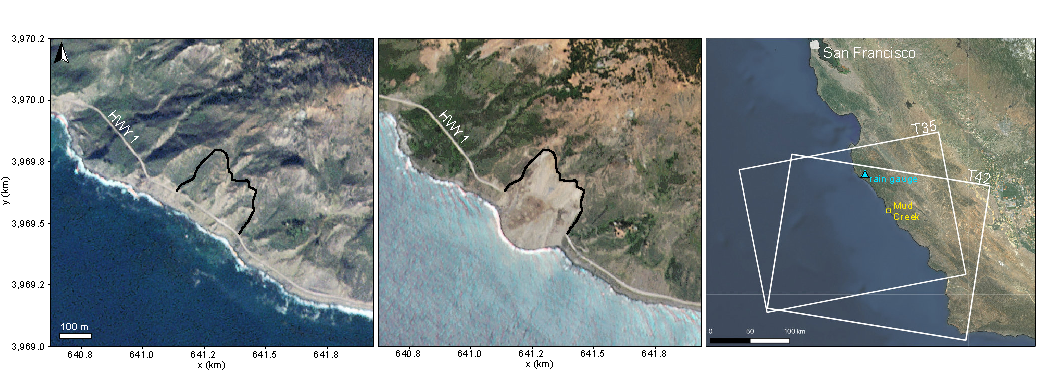
\includegraphics[width = \textwidth]{OverviewFigure_2.pdf}
    \caption{Big Sur coast with Highway 1 before and after the Mud Creek landslide (left and center, x and y coordinates in UTM Zone 10 N. Images from © \cite{planetteam2017}), and landslide and rain gauge locations and Sentinel-1 ascending (T35) and descending (T42) orbit footprints (right; basemap from ESRI World Imagery - Source: Esri, Maxar, GeoEye, Earthstar Geographics, CNES/Airbus DS, USDA, USGS, AeroGRID, IGN, and the GIS User Community)}
    \label{fig:overview}
\end{figure}


\section{Methods and data}
\label{sec:methods}
For the analyses presented here, we worked with both radar and optical images: We used data from ESA's C-band Sentinel 1A and 1B radar satellites (5.6\,cm wavelength) and processed 51 images from the ascending orbit (track 35) and 63 from the descending orbit (track 42). Single Look Complex (SLC) images were obtained from the Alaska Satellite Facility (ASF DAAC: \url{https://search.asf.alaska.edu}). Because we focused this study on pre-failure landslide dynamics, we did not include any post-landslide radar images in the analysis. To compute the NDVI, we downloaded 22 cloud-free Sentinel-2 images (10\,m resolution) from the U.S. Geological Service's (USGS) Earth Explorer platform (\url{https://earthexplorer.usgs.gov/}). We used both datasets to compute time series of ratios that describe the discrepancy between the behavior of the landslide and its surrounding slope. The advantage of the ratio calculation is that it cancels out the effects of regional-scale environmental factors and processing artefacts that affect the hillslope and the landslide equally. Therefore, when using the landslide/hillslope ratio, values less than 1 indicate decreasing landslide NDVI or coherence values, while values greater than 1 indicate decreasing hillslope values. Table \ref{tab:products} shows an overview of the raw data products and associated derivatives (details are given in the sections below). 


\begin{table}[hbt]
    \centering
     \caption{Overview of data products used in this study and the number of products derived at the different processing steps.}
    \begin{tabular}{c| c c c c c}
    Product & SLC images & Cloud-free NDVI images & Interferograms & Ratio processing  & Displacement processing \\ 
    \hline
         Sentinel-1 ascending & 51 & - & 172 & 132 & -\\
         Sentinel-1 descending & 63 & - & 208 & 141 & 193\\
         Sentinel-2 & 22 & 22& -& 22 & -\\ 
    \end{tabular}
    \label{tab:products}
\end{table}

\subsection{Radar background}
%SAR images contain measurements of backscatter amplitude and radar phase for each point on the ground. Radar backscatter is the amount of energy reflected back to the sensor from each ground point. It is influenced by the geometry of the target, its surface roughness, and dielectric properties \citep[e.g.,][]{massonnet1998}. InSAR uses the change in the phase of radar waves between measurements to quantify changes at the Earth's surface.
\par
Two SAR images acquired by the same satellite of a given area at different times can be processed into interferograms: images that represent the phase difference [0,$2\pi$] between the two acquisitions at each point. In the initial interferogram, the phase differences contain contributions from the varying orbital geometries, topography, atmospheric path delays and surface displacements. After removing the effects of viewing geometry, topography and atmosphere, and with knowledge of the radar wavelength, these phase changes can be converted to surface displacements \citep[e.g.,][]{massonnet1998, rosen2000, wasowski2014}. Because InSAR is sensitive to deformation only in the instrument's line of sight (LOS), three independent measurements are required to obtain the true 3-D motion of a target. In the absence of independent measurements, LOS deformations can be projected onto the downslope direction by assuming that the primary motion of a landslide follows gravity (see section \ref{sec:disp} and Fig. \ref{fig:los}).     
\par  
Alongside any computed interferogram is a coherence $(\gamma)$ image that serves as the primary quality indicator for InSAR data. It is a measure of how similar the ground properties are at the time of the radar acquisitions \citep{scott2017, zebker1992}, and is computed from the local phase variance in the interferogram. Given the stable imaging geometries of Sentinel-1 data, coherence changes are expected to be almost exclusively due to temporal variability. On a vegetated, active landslide, coherence is likely controlled by three factors: \par

First, coherence is affected by the surface geometry. The resulting phase of any pixel is the coherent sum of all scatterers within that pixel, and when the geometry of those scatterers changes substantially, the resulting phase changes. Therefore, both changing vegetation and erosion can lead to a loss of coherence \citep{massonnet1998, rosen2000, ruescas2009}. In the non-landslide context, this is effect is visible when fields are plowed, crops are harvested, or snow falls between two image acquisitions, to name just a few examples.\par
Second, displacements that surpass the temporal and/or spatial aliasing thresholds, even if they do not alter the surface geometry, lead to a loss of coherence \citep[e.g.,][]{massonnet1998, rocca2000, zhou2009, wasowski2014, manconi2018}. This effect can be well visible on fast moving glaciers \cite[e.g.,][]{joughin1996}.\par
Lastly, soil moisture may be affecting the coherence, because it can alter radar phase and backscatter. This effect has been shown in many studies, but the reasons for this are still debated. Soil moisture variations may change the phase response (and backscatter amplitude) by influencing the penetration depth of radar waves, with drier soils allowing deeper penetration. This influences the number of scatterers controlling the phase and backscatter amplitude in any given pixel. Therefore, interferograms created from images with varying soil moisture contents may decorrelate due to the altered number of scatterers. In addition, if soils expand or contract with changing moisture, changing the distance to the radar instrument, the phase response may also be altered, leading to lower coherence \citep{scott2017, rabus2010, nolan2003, ulaby1996}. Recent studies, however, suggest that coherence loss is better explained by the filling of pore space with water, which increases the dielectric constant, which in turn increases the wavenumber in the soil \citep{eshqimolan2020, zwieback2015}. \par

\subsection{Radar processing}
We processed the InSAR data using JPL's InSAR Scientific Computing Environment (ISCE; \cite{rosen2012}). SAR images for our study site were available beginning in April 2015, with images typically acquired every 12 days (a few pairs with 6 day spacing were available). We allowed for a maximum time difference of 48 days between images and produced 172 interferograms from the ascending orbit and 208 from the descending orbit (see Table \ref{tab:products}). A gap in the ascending data between late 2015 and early 2016 led us to increase the permissible time difference between images in that period to one year (maximum resulting temporal baseline = 342 days). Because the study site is relatively small compared to the native spatial resolution of the SAR imagery, we downsampled the images to two looks in range and one look in azimuth, and removed the topographic phase with the USGS's 1/3 arc second DEM, the highest resolution seamless DEM available for the conterminous United States (downloaded from: \url{https://viewer.nationalmap.gov/basic/}). Due to the small size of our area of interest, we did not perform any tropospheric or ionospheric corrections. We unwrapped the interferograms using the statistical-cost, network-flow phase-unwrapping algorithm (SNAPHU; \cite{chen2002}) and applied a standard power spectral filter (value 0.5) to reduce the phase noise \citep{Goldstein1998}. We subsequently used the generated coherence images and unwrapped interferograms for this study.

\par Decisions about the quality of an interferogram and the reliability of the data for time series analyses are usually based on radar coherence. For individual interferograms, pixels with a coherence of less than 0.2 are typically masked \citep[e.g.,][]{rosen2000}. Images with low overall coherence are usually omitted from InSAR time series analyses. This selection is often based on visual inspection and performed manually \citep[e.g.,][]{handwerger2019}. To increase the reproducibility of our work, we experimented with a set coherence threshold that we used to filter out poor quality interferograms. Because our area of interest is small relative to the size of the interferogram, mean image coherence over the entire interferogram is a poor indicator for the data quality in the landslide area. Instead, we calculated the mean coherence for each interferogram within just our area of interest and only retained images with a mean coherence above a defined threshold (0.35 for the displacement analysis and 0.5 for the coherence ratio analysis; see details in sections \ref{sec:disp} and \ref{sec:coh}). Fig. \ref{fig:coherence_filter} illustrates why relatively aggressive filtering is necessary for the ratio calculations. If the entire area of interest is affected by low coherence, the ratio becomes meaningless. After filtering, we computed the time series of displacement and radar coherence ratio from all the retained images. \par 


\subsubsection{Coherence ratio}
 \label{sec:coh}
To construct a time series of coherence evolution, we filtered out all interferograms with mean coherence of less than 0.5 in our area of interest (Fig. \ref{fig:coherence_filter}). This higher threshold was necessary to detect any differences between the unstable part of the slope and the surrounding area. In cases where the coherence of the entire area is low, the ratio value becomes meaningless. We retained 132 interferograms from the ascending track and 141 interferograms from the descending track after applying this filter criterion (Tab \ref{tab:products}).\par 
ISCE computes coherence using a 5 x 5 pixel triangular weighted window. For signals $s_1$ and $s_2$, coherence is given by
\begin{equation}
    \gamma = \frac{\lvert \langle s_1 s^*_2\rangle\rvert}{\sqrt{\langle s_1 s^*_1\rangle \langle s_2 s^*_2\rangle}}\qquad 0\leq | \gamma | \leq 1,
\end{equation}
where * indicates the complex conjugate \citep{jung2016}.\par
We created a time series of radar coherence ratio ($C_R$) by calculating the ratio between the mean coherence over the slide (the area that ultimately failed) and the mean coherence over the surrounding slope (termed Reference Slope, see Figure \ref{fig:coh_evolution}) as:\par
\begin{equation}
    C_R=\frac{\overline{\gamma}_{Slide}}{\overline{\gamma}_{RefSlope}}
\end{equation}
Figure \ref{fig:coh_evolution} shows the evolution of the coherence in the area of interest as well as the polygons used to calculate the mean coherence on the slide and the surrounding hillslope for four interferograms acquired in the fall of 2016 and spring 2017. For the slide polygon, we mapped the area that failed in the landslide. The reference hillslope was mapped as the area immediately surrounding the landslide with similar slope, aspect and vegetation cover. \par

%In an equivalent manner, we compared the radar backscatter intensity between the landslide and the surrounding hillslope in order to investigate possible variations in soil moisture between  
%\begin{equation}
%    A_R=\frac{\overline{\sigma}^0_{Slide}}{\overline{\sigma}^0_{RefSlope}},
%\end{equation}
%where $\overline{\gamma}_{Slide}$ and $\overline{\sigma}^0_{Slide}$, and $\overline{\gamma}_{RefSlope}$ and $\overline{\sigma}^0_{RefSlope}$ are the mean values of radar coherence and backscatter over the slide and reference slope, respectively. This calculation is advantageous because it eliminates the effect of coherence loss due to increasing temporal and spatial baselines, regional-scale atmospheric disturbances, or vegetation cycles. Because these factors are expected to affect the larger region, any deviation from a ratio of 1 indicates varying behaviors between the landslide and the surrounding hillslope. The reference slope was determined from optical images and a DEM to include the hillslope immediately surrounding the landslide and has a similar aspect, slope and vegetation cover.  

\begin{figure}
    \centering
    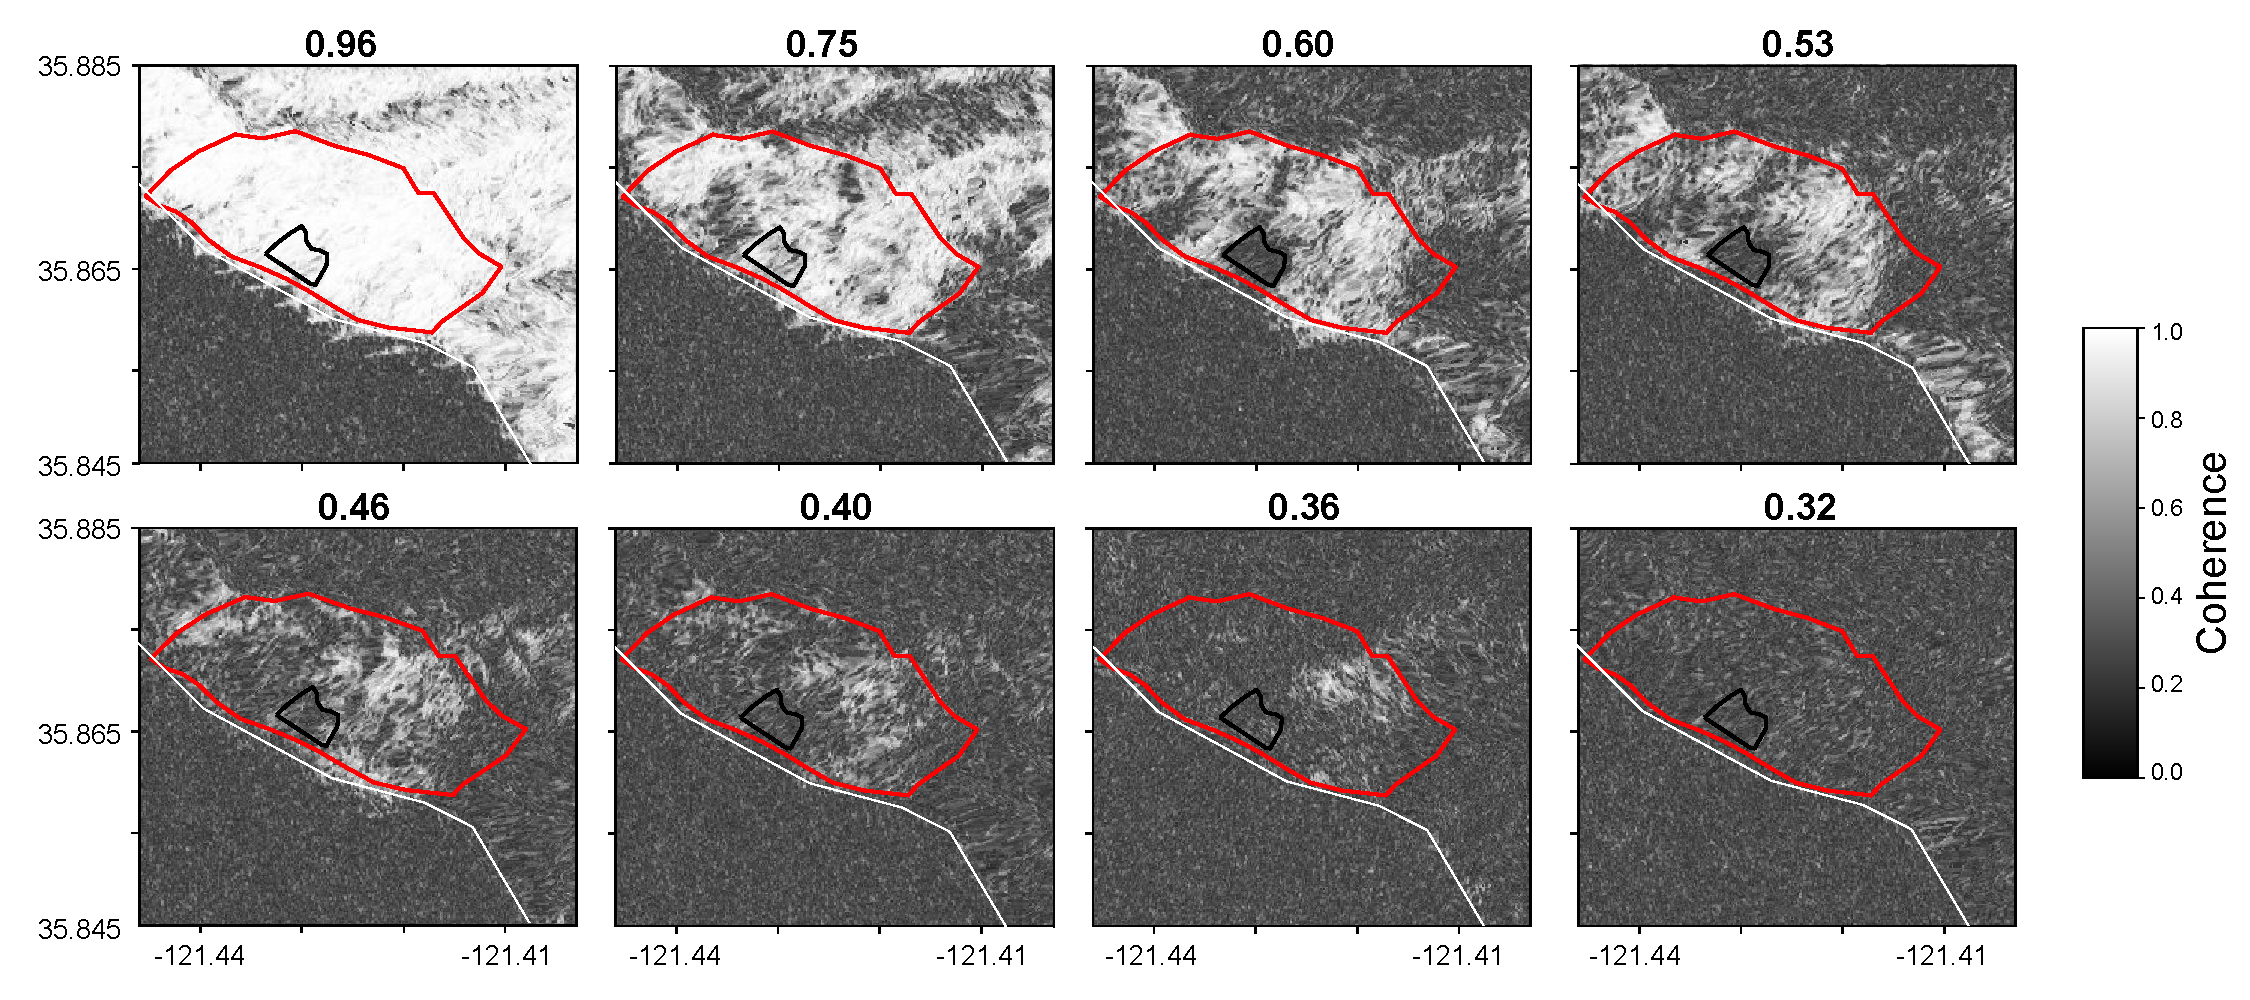
\includegraphics[width = \textwidth]{coherence_filter_sample_1.pdf}
    \caption{Coherence filtering: Interferograms in the upper row exceed the coherence threshold of 0.5 and were therefore included in the ratio analysis, the images in the lower row were excluded. We calculated the mean coherence for the area in the red polygon. The images represent various times throughout the the two year period for which data was available and were chosen purely to show why low mean coherence images cannot be used for the ratio calculation. The 20 May 2017 landslide occurred inside the black outline (corresponding to dashed gray line in Fig. \ref{fig:displacement}). Coherence derived from Copernicus Sentinel-1 data.}
    \label{fig:coherence_filter}
\end{figure}

\begin{figure}[hbt!]
    \centering
    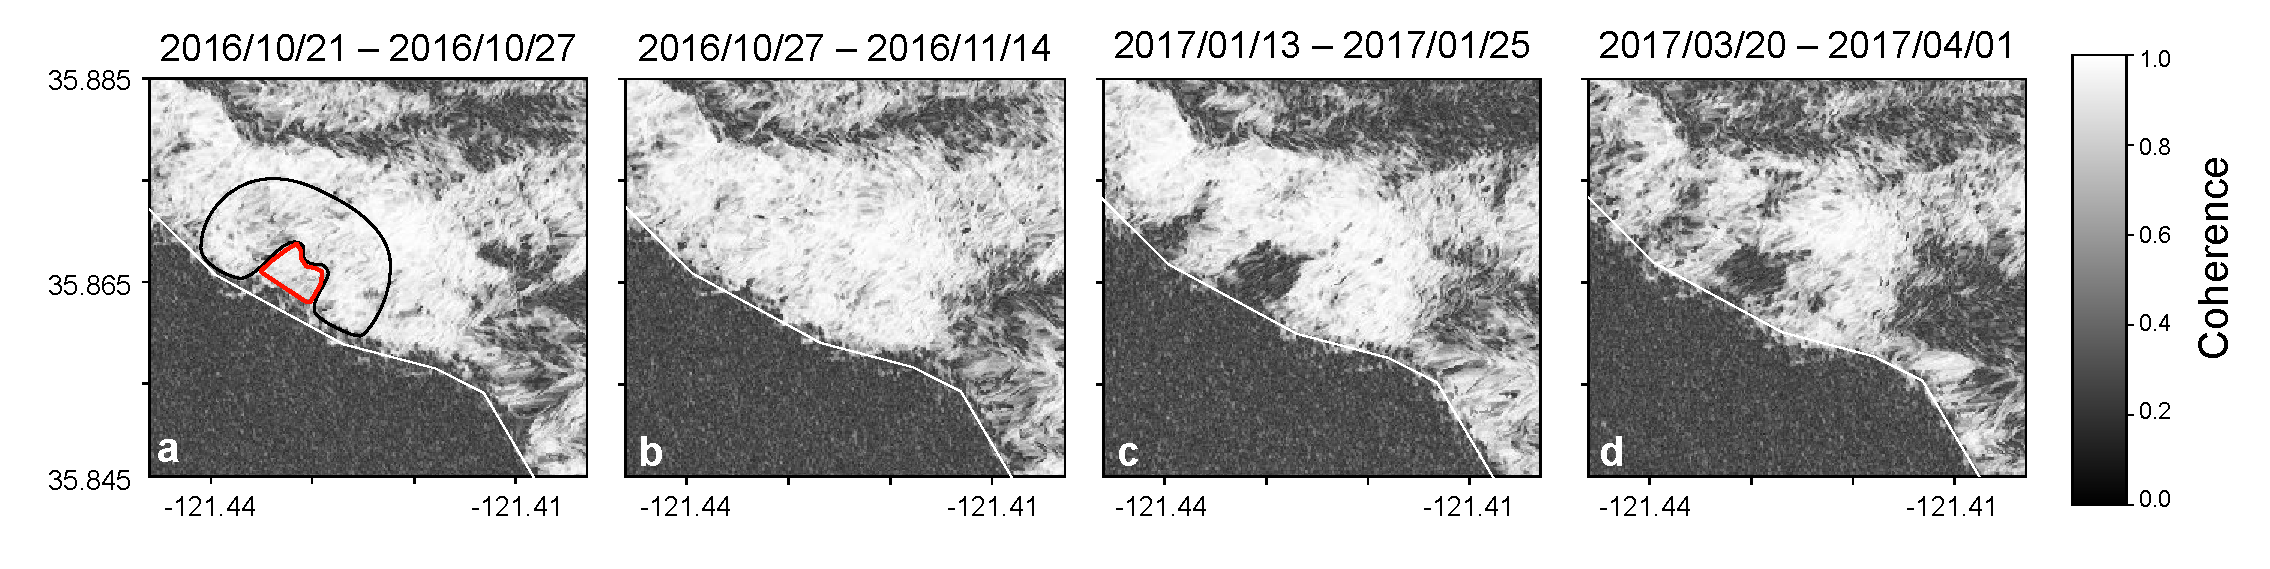
\includegraphics[width = \textwidth]{coherence_evolution_1.pdf}
    \caption{Interferometric coherence of the Mud Creek landslide and surrounding slope in Fall 2016 (a \& b) and Spring 2017 (c \& d). the landslide outline is marked in red, and the coherence loss in that area is clearly visible in panels c and d. The reference hillslope is outlined in black. Coherence derived from Copernicus Sentinel-1 data.}
    \label{fig:coh_evolution}
\end{figure}

\subsubsection{Displacement}
\label{sec:disp}
To complement the coherence ratio time series we also computed a displacement time series. For this part of the analysis, we used only the interferograms from the descending track that had a mean coherence of more than 0.35 in our area of interest. This produced a fully connected time series with 193 interferograms (Tab. \ref{tab:products}). The ascending data does not lend itself to measuring the displacement because the local incidence angle is around 90\textdegree, leading to minimal motion in the satellites line of sight. We selected a point west of the landslide as our stable reference region. This area is the same geologic unit, its vegetation cover is representative of the larger area, and it did not fail in the landslide. A preliminary displacement analysis also suggested it had not experienced any significant deformation. We computed the displacement time series using the New Small Baseline Subset (NSBAS; \cite{berardino2002}) method implemented in JPL's Generic InSAR Analysis Toolbox (GIAnT; \cite{agram2013}) and applied a coherence threshold of 0.3 to mask individual low coherence pixels. We then retrieved surface displacements by projecting the measured line of sight deformation at each point onto the fall line. To do this we defined the unit line of sight vector \textit{a} to point from the satellite to the target and the unit fall line \textit{b} to point from target down slope along the steepest gradient. We describe both vectors in a polar coordinate system where $\theta$ describes a positive counter-clockwise rotation from x (east), and $\phi$ describes the angle from positive up (Fig. \ref{fig:los}). The full slope parallel deformation $D_t$ could then be retrieved as
\begin{equation}
    D_t = \frac{LOS}{cos(\delta)}, 
    \label{eq:los1}
\end{equation}
where LOS is the measured line of sight deformation and $\delta$ is the angle between \textit{a} and \textit{b}, which is defined as:
\begin{equation}
    cos(\delta) = \frac{a \cdot b}{\rvert a \rvert \rvert b \rvert}
    \label{eq:los2}
\end{equation}
  
\begin{figure}[hbt!]
    \centering
    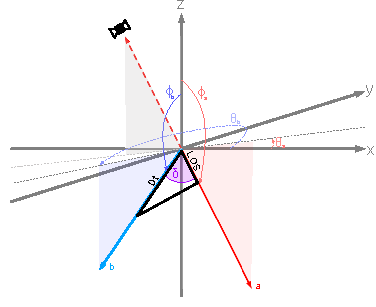
\includegraphics[scale = 1.5]{los_projections.pdf}
    \caption{Vector geometries used to project measured line of sight displacements (\textit{LOS}) onto the fall line (\textit{b}). For \textit{a} and \textit{b}, $\theta$ describes the azimuth from x (East) and $\phi$ describes the angle from positive up. The angle $\delta$ between \textit{a} and \textit{b}, controls how much of the true deformation is visible in the satellites LOS.}
    \label{fig:los}
\end{figure}  

\subsection{Optical data}
To investigate the extent to which coherence variability may have been driven by changes in vegetation cover, we computed a time series of Normalized Difference Vegetation Index (NDVI) from 22 ESA Sentinel-2 optical images (Tab. \ref{tab:products}) acquired between 4 December 2015 and 27 May 2017. NDVI is a measure of vegetation productivity that can be derived from the red  and near infrared (NIR) channels in optical imagery (bands 4 and 8 in Sentinel-2):  \par

\begin{equation}
    NDVI = \frac{{NIR - red}}{{NIR + red}}
\end{equation}

NDVI makes use of the fact that photosynthetically active vegetation is bright in the near infrared spectrum ($\lambda \sim$800 nm) and dark in the red wavelengths ($\lambda \sim$600 nm; \cite{tucker1979, carlson1997}). The index values vary between -1 and 1, where denser and/or more productive vegetation results in more positive values and sparse vegetation or bare ground results in low or negative values. Typical values for dense, healthy vegetation are around 0.6, values for bare ground or minimal vegetation are typically below 0.2 \citep{jensen2009}. We calculated the NDVI for all available cloud-free images back to December 2015 and then computed our time series in the same manner that we did for coherence ratios: \par
\begin{equation}
    NDVI_R= \frac{\overline{NDVI}_{Slide}}{\overline{NDVI}_{RefSlope}}
\end{equation}
In addition to the time series of NDVI ratio, we thresholded all NDVI images at a value of 0.25 and investigated the spatial changes through time.  
\subsection{Precipitation data}
Precipitation data were obtained from the National Oceanic and Atmospheric Administration's (NOAA) Global Historical Climate Network Daily (GHCND) platform. GHCND data provide daily total cumulative precipitation and minimum and maximum air temperature. The Big Sur Station station is located 53 km north-west of Mud Creek at 61 m asl. Data is available from \url{https://www.ncdc.noaa.gov/cdo-web/datasets/GHCND/stations/GHCND:USC00040790/detail} and were used without any additional processing. % the Hearst Castle station is located 31 km south-east of Mud Creek at an elevation of 465 m asl. %In order to investigate the spatial precipitation patterns, we acquired NASA IMERG data. We compared IMERG precipitation time series from Mud Creek, Big Sur Station, and Hearst Castle to each other as well as to the GHCDN station data. 

\section{Results}
\label{sec:results}
\subsection{Coherence ratio}
The results of coherence ratio analysis are shown in Fig. \ref{fig:coherence_timeseries}, alongside the NDVI time series and the precipitation record. The 132 good quality interferograms from the ascending orbit form a mostly-continuous time series, though there was a gap in data acquisition in late 2015 and early 2016. The descending track offers a more continuous time series between 2015 and early 2017 (longest temporal baseline = 48 days), but few interferograms from 2017 passed the coherence threshold. The coherence ratio hovers around 1 throughout the dry seasons in both datasets. In spring 2016, following a short period of intense rainfalls, the coherence ratio calculated from ascending data drops to around 0.8 and only recovers slowly. This drop is less distinct in the descending data. Then, coincident with a large increase in cumulative precipitation in early 2017, the coherence ratio drops markedly to around 0.6 and does not recover until the catastrophic failure of the landslide.  \par
%The amplitude time series on both the ascending and descending tracks show some seasonal trends, but there is no clear difference between 2017 and earlier years. It appears that there is little difference between the backscatter received from the slide body and the surrounding slope in the descending track. Conversely, the backscatter received from the slide body on the ascending track is higher than that of the surrounding slope.  

\begin{figure}[hbt!]
    \centering
    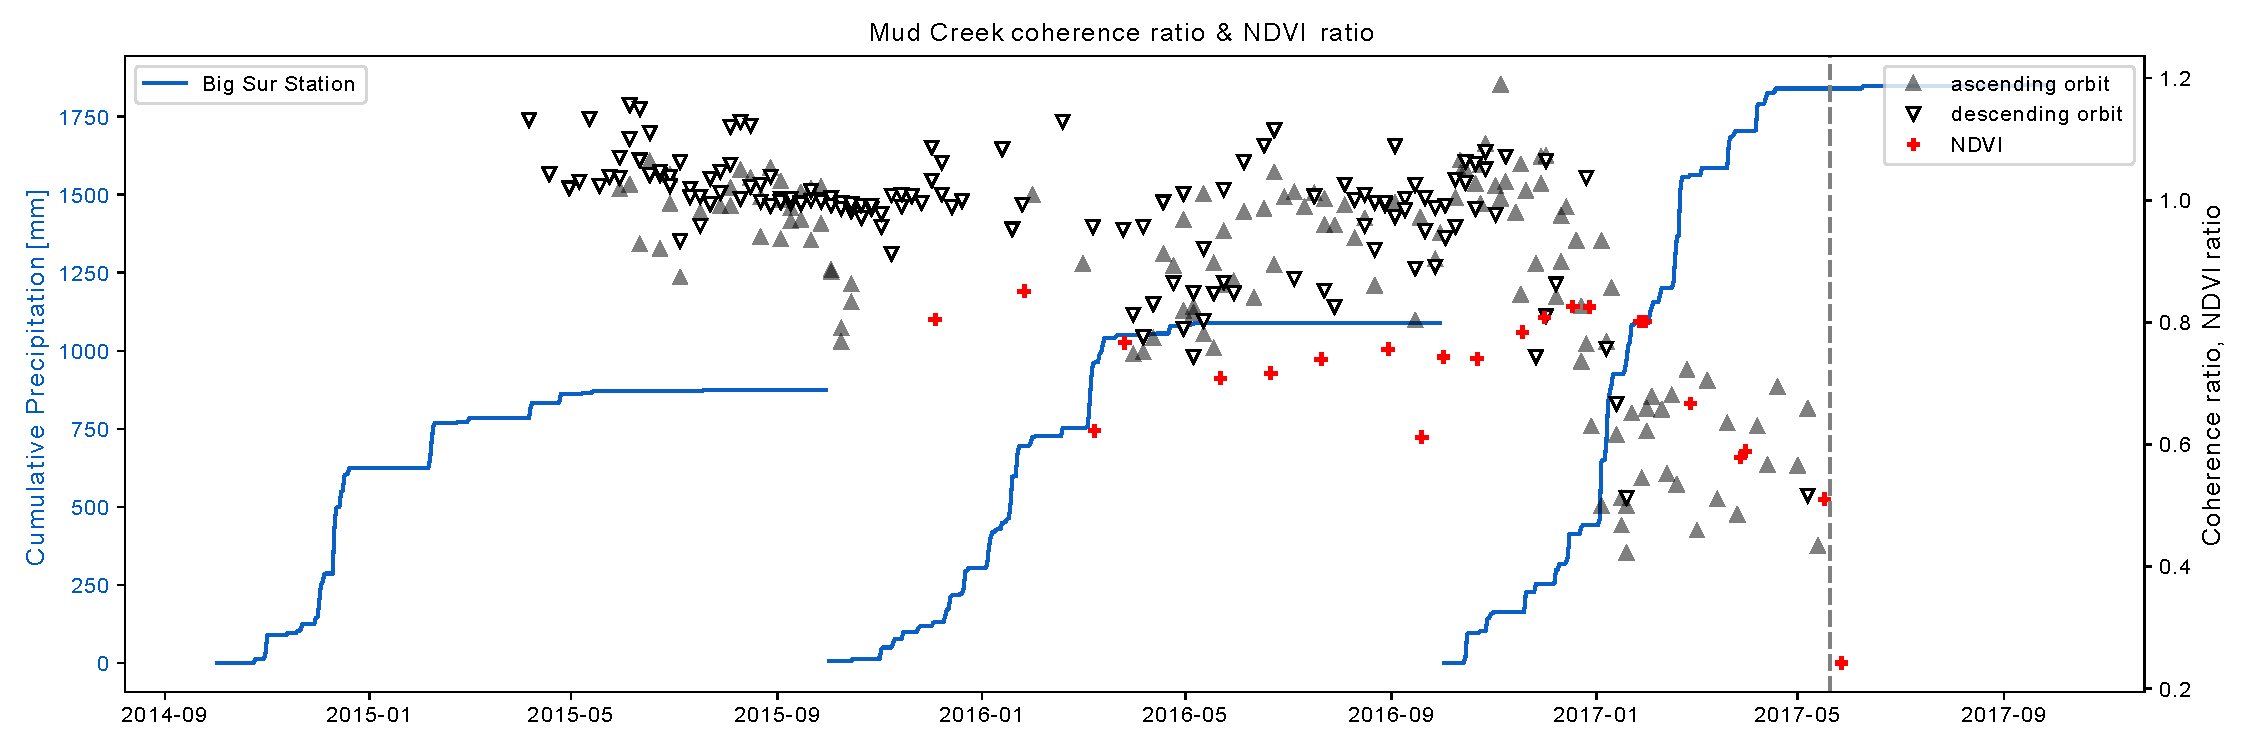
\includegraphics[width = \textwidth]{coherence_ndvi_2.pdf}
    \caption{Radar \textbf{coherence} ratio plotted against NDVI ratio and cumulative precipitation (at Big Sur Station). The dashed line indicates the timing of the landslide. The coherence-ration hovers around 1 for most of the time prior to the failure, before dropping starkly in January 2017. At the same time, the NDVI ratio begins a gradual decline. A similar behavior for both indices is visible in March 2016.}
    \label{fig:coherence_timeseries}
\end{figure}

%\begin{figure}[hbt!]
%    \centering
%    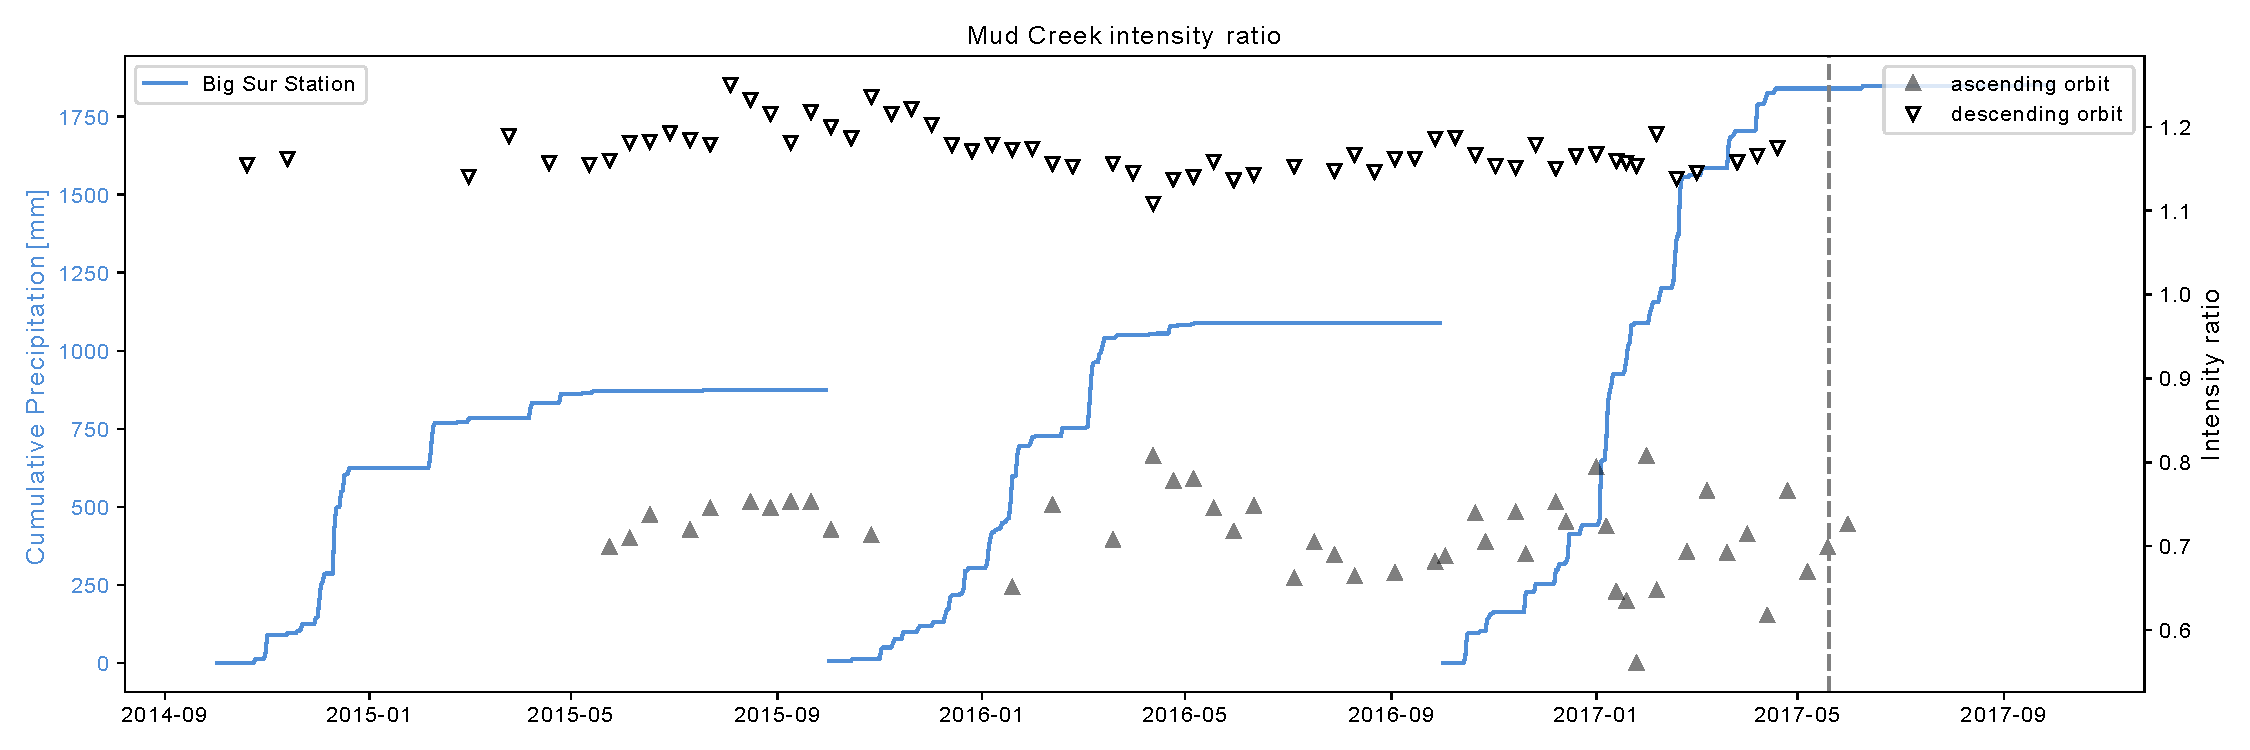
\includegraphics[width = \textwidth]{intensity_ratio.pdf}
%    \caption{Radar \textbf{amplitude} ratio plotted against NDVI ratio and cumulative precipitation (at Big Sur Station). The dashed line indicates the timing of the landslide.}
%    \label{fig:amplitude_timeseries}
%\end{figure}



\subsection{NDVI}
The NDVI, NDVI ratio, and the changes in the spatial pattern also show that processes ongoing on the landslide differed substantially from the surrounding slope. The NDVI ratio of 0.8 prior to 2017 indicates that the Mud Creek slope is generally less densely vegetated than the surrounding hillslope (Fig. \ref{fig:coherence_timeseries}). This observation is also supported by the raw NDVI time series which indicates that NDVI values on the landslide vary seasonally between around 0.2 and 0.4, while ranging from about 0.25 to 0.5 on the surrounding hillslope (Fig. \ref{fig:ndvi_noratio}). These individual time series reveal that the evolution of the vegetation cover on the slide closely paralleled that of the surrounding slope throughout 2016, with productivity peaking in April. In early 2017, we observe a clear divergence of the two time series, as vegetation productivity in the slide area began to decline, before plummeting post-slide. These time series demonstrate that the evolution of the NDVI ratio is in fact controlled by a decrease of vegetation productivity or coverage on the slide and not an unusual increase of productivity on the reference slope (Fig \ref{fig:ndvi_noratio}). 
The gradual decline of the NDVI ratio starting in early 2017 therefore suggests that vegetation cover on the landslide was degrading. When comparing this to the spatial evolution of NDVI values, it is evident that low NDVI regions on the slide were expanding throughout the spring of 2017, driving the decrease in mean NDVI. A low NDVI area, which can be attributed to a steep gully, is consistently present in the center of the slide (see panel typical pattern in Fig. \ref{fig:ndvi_pattern}). The panel from March 8 in Fig. \ref{fig:ndvi_pattern} shows that the drop in NDVI ratio observed in spring 2016 can also be linked to a large expansion of the low NDVI area (Fig. \ref{fig:coherence_timeseries}). This drop also corresponded to one of the largest rainfall events witnessed that year. The low NDVI ratio in September 2016 is caused by a cloud bank obscuring the toe of the slide, and is therefore not associated with an actual change of vegetation. Then, throughout the spring of 2017, the low NDVI values expanded, driving the decreasing mean NDVI until all vegetation was removed due to the failure of the slope (see post-slide image from 27 May 2017 in Fig. \ref{fig:ndvi_pattern}).    \par
 
\begin{figure}[hbt!]
    \centering
    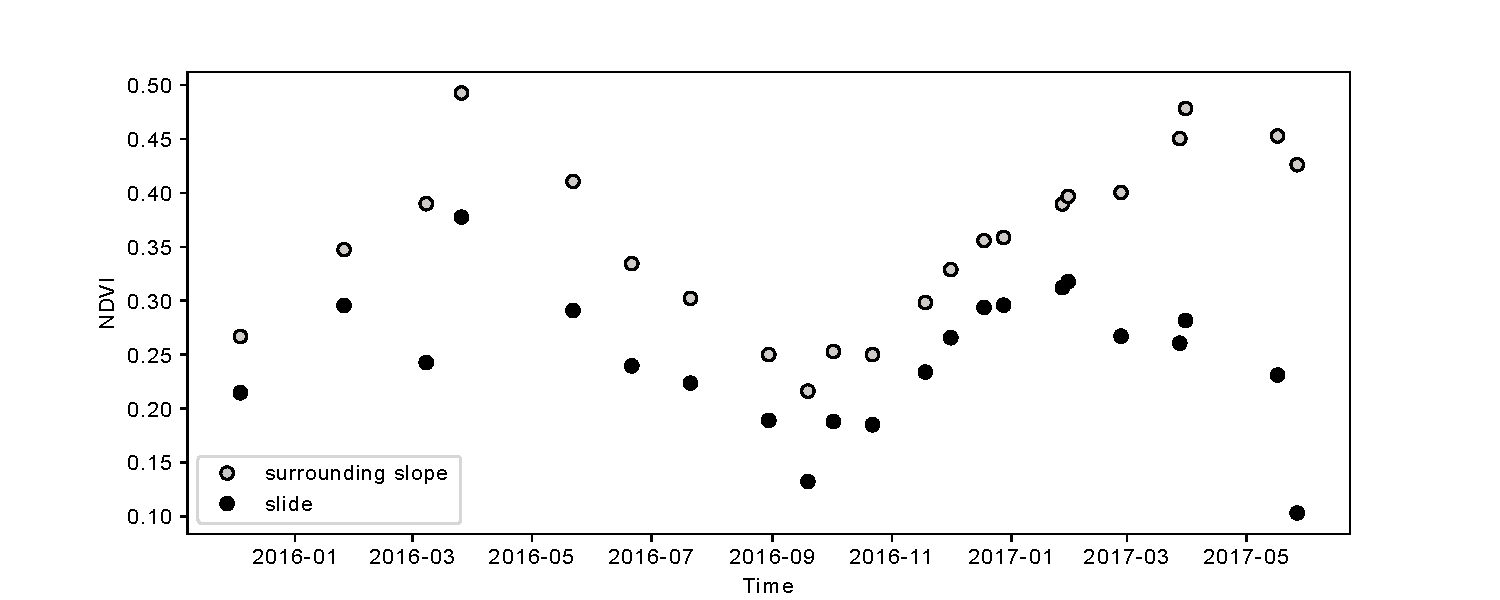
\includegraphics[scale = 0.5]{NDVI_noratio.pdf}
    \caption{NDVI on the Mud Creek slide body and the surrounding slope. Note that the last data point in May 2017 is from an image acquired after the landslide.}
    \label{fig:ndvi_noratio}
\end{figure}

\begin{figure}[hbt!]
    \centering
    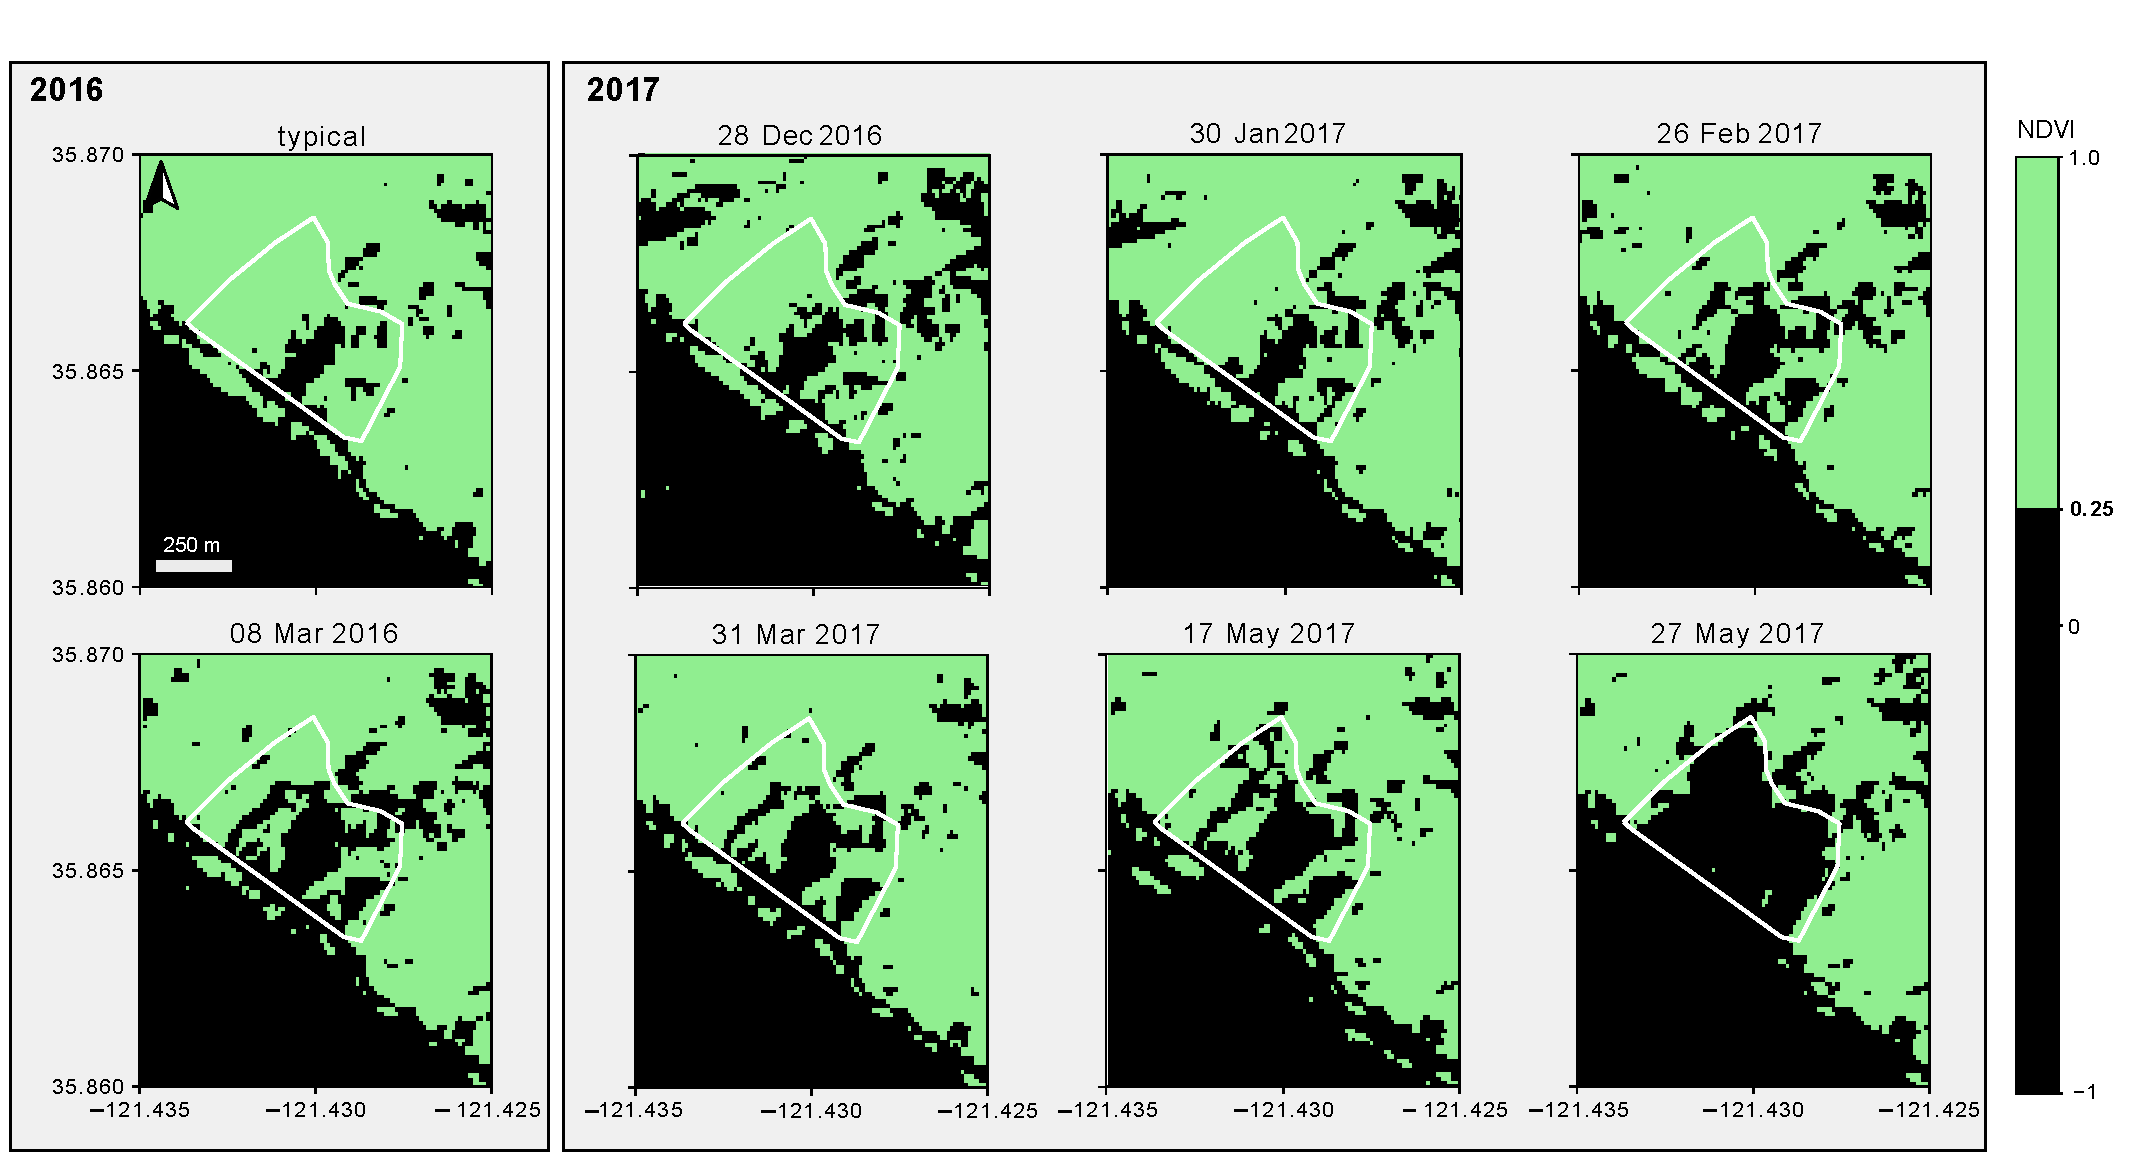
\includegraphics[scale = 0.5]{ndvi_patterns_fig_0.25.pdf}
    \caption{NDVI on the Mud Creek landslide. The first panel shows the pattern that is typical (example from 26 March 2016). The 8 March 2016 panel corresponds to the dip in NDVI ratio visible in early 2016. The area of low NDVI grows ever larger during the spring of 2017, before much of the vegetation is removed during the landslide (post-slide image from 27 May 2017).}
    \label{fig:ndvi_pattern}
\end{figure}


\subsection{Deformation}
%Because InSAR only detects the component of motion in its line of sight, the local incidence angle critically controls how much motion the radar can see. At Mud Creek, the radar's line of sight on the ascending orbit intersects the fall line at a near right angle in most places, impeding the detection of downslope motion. 
On the descending orbit, the line of sight intersects the fall line at a favorable angle that allows us to retrieve about 50\% of the total displacement. To retrieve a more accurate record of true deformation we projected the measured line of sight displacements onto the downslope direction as described in equations \ref{eq:los1} and \ref{eq:los2}.\par 
Figure \ref{fig:displacement} shows the slope parallel displacement obtained from the descending track. The total cumulative displacement on the Mud Creek landslide since April 2015 (beginning of Sentinel-1 measurements) ranges from $\sim$0.15\,m to $\sim$0.55\,m. The displacement time series at three different points show the large acceleration that took place in spring 2017. The time series from the reference region (solid line in Fig. \ref{fig:displacement}) confirms that the area around the landslide was stable throughout the entire time period. At several points in time, the cumulative displacement reverses direction, indicating that unwrapping errors hamper the retrieval of the true displacement. This behavior is particularly obvious during the 2017 speedup, but also during the spring of 2016 (line with stars if Fig. \ref{fig:displacement}). The area showing measurable displacements is somewhat larger than the area that failed on May 20th, but smaller than the area that consistently showed low coherence in the months preceding the landslide (dashed lines in Fig \ref{fig:displacement}).

\begin{figure}[hbt!]
    \centering
    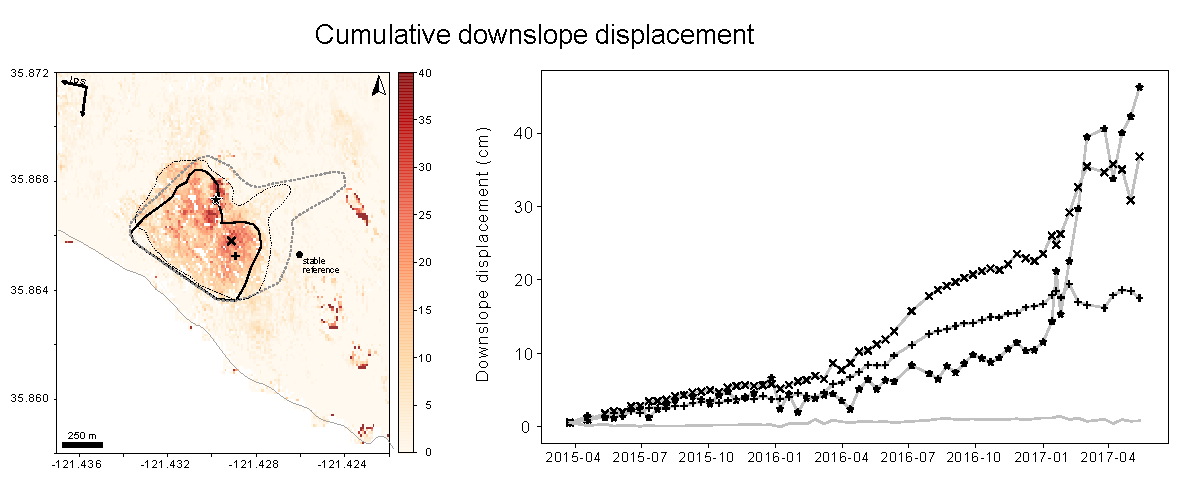
\includegraphics[width=\textwidth]{MudCreekDownslopeDisplacement_3_losarrow.pdf}
    \caption{Left: Cumulative line of sight displacements from April 2015 to May 2017 projected onto the fall line. The solid black line indicates the extent of the slope that failed, the dashed black line the area showing significant displacement, and the dashed grey line the area of low coherence. Right: Time series of displacement at three different points within the slide (indicated by the $\bigstar$, $\times$ and + signs) as well as in the region used as stable reference (solid line). }
    \label{fig:displacement}
\end{figure}

\section{Discussion}
\label{sec:discussion}
%Assessing landslide activity is a central part of hazard management and can provide critical information about the stability of a hillslope \citep{vanwesten2006}. Here, we applied a slight twist to radar coherence and NDVI analyses, measures that are typically used for post-failure landslide mapping, by comparing mean values of coherence and NDVI on the landslide to the surrounding, stable hillslope. We created time series of these data to investigate their usefulness for assessing landslide activity. 
Five months before its final failure, in conjunction with some of the largest rainfall events measured during California's 2016/2017 winter season, the coherence ratio over the Mud Creek landslide dropped suddenly. At the same time, the NDVI ratio began a near linear decline (see Figure \ref{fig:coherence_timeseries}). These data raise the question of how and if they can useful indicators of landslide activity, what challenges this new analysis poses, and what its limitations are. \par

%Coherence ratio paragraph
The fact that fewer interferograms from the descending track passed the coherence threshold can likely be explained by the differences in viewing geometries: The ascending track is right-looking, causing the radar waves to intersect the hillslope at a near right angle. Conversely, on the descending track (also right looking), the radar waves intersect the hillslope at an oblique, near surface-parallel angle. This oblique viewing geometry makes the radar waves more susceptible to volume scattering on vegetation \citep{massonnet1998}. Indeed, we see wide-spread areas of low coherence during the growing season in the data from the descending track. Unfortunately, the period leading up to the landslide is most impacted by this effect, while data from the ascending track is much less affected. Despite this discrepancy, the pre-failure coherence drop is visible in the data from both orbits. The coherence loss therefore cannot be attributed to geometric differences, but must represent a change on the ground.\par

The power of the ratio calculation lies in its capability to cancel out negative effects of long temporal baselines, as well as regional atmospheric and environmental changes. If the slope and surrounding hillslope have similar scattering properties, then environmental and atmospheric changes that affect InSAR coherence (e.g., vegetation cycles, precipitation events, ionospheric disturbances) will not differ between a landslide and its surrounding slopes. At Mud Creek, this similarity is given because neither of the slopes are used for agriculture, nor is there any form of human development. Furthermore, both slopes cover a similar altitude range, slope and aspect; optical images suggest they have a very similar vegetation cover (Fig. \ref{fig:overview}); and the geologic map of the area indicates that the entire area is part of the Franciscan Mélange \citep{californiageologicsurvey}. In this manner, as long as coherence is maintained in some part of the area of interest, interferograms with varying temporal baselines can be compared to gain insight into governing processes. \par


The drop of the coherence ratio in the time series is a clear indicator of ongoing changes by itself, but is useful to consider what factors might be driving these changes in order to understand the value of the coherence ratio with regard to assessing landslide activity. The coherence images (Fig. \ref{fig:coh_evolution}) show clearly that the coherence on the slide dropped drastically, therefore we attribute the effect of the dropping ratio entirely to changing conditions on the slide. However, the change in coherence could be caused by changes to soil moisture, vegetation changes, erosion and active deformation - all of which are processes that may be ongoing on an actively deforming slope that ultimately failed due to increasing pore water pressure \citep{handwerger2019}. As we try to parse out the different influences on coherence ratio, it is important to note that more than one factor may be the leading cause at any given time, and their relationship may vary through time. Disentangling the causes of the coherence drop is therefore by no means straightforward. \par


%NDVI paragraph
The NDVI ratio began its near linear decline in the spring of 2017, concurrent with peak precipitation and the observed drop in the coherence ratio. Fig. \ref{fig:ndvi_noratio} clearly shows that the drop of the NDVI ratio can be attributed to changes that are occurring on the slide and not on the surrounding slope. Indeed, during the spring of 2017, more and more pixels in the slide area showed an NDVI of less than 0.25, indicating that the removal or degradation of healthy vegetation was impacting a larger and larger area. However, the pattern seen on 17 May 2017, just three days before the failure, hardly differs from that on 8 March 2016, suggesting that the Mud Creek landslide had experienced this type of vegetation degradation before. Given this similarity, is likely that the same process led to the low NDVI in 2016 and in 2017. The fact that in 2016 the NDVI ratio recovered within just 18 days (8 March to 26 March) suggests that vegetation was not completely removed.  If vegetation was not, or only partly, physically removed, covering of plants with mud from ongoing erosion could explain the low NDVI. Whether the vegetation cover was destroyed or just coated in mud, both processes point to an increased activity of the landslide. \par


% Displacement and Unwrapping Errors Paragraph
The deformation analysis of the Mud Creek landslide shows a significant acceleration prior to failure. However, the displacement time series presented here fails to pick up the period of acceleration in 2016 reported by \cite{handwerger2019}. This is not surprising given that unwrapping errors, the effect of which we see throughout the time series, can make measuring the true surface velocities particularly difficult for fast moving and accelerating landslides \citep[e.g.,][]{handwerger2019, dai2020, manconi2018}. Unwrapping errors can be reduced by subtracting the mean landslide velocity prior to the phase unwrapping, which can reveal the missing phase cycles and help recover more of the true deformation \citep{handwerger2015, handwerger2019}. However, this approach requires assessing each landslide individually, and does not lend itself to automatic processing at large scales. We did not apply a correction to subtract the mean landslide velocity and are therefore not able to recover the full deformation. Nevertheless, our $\sim$0.6\,m cumulative surface displacement measurements are in good agreement with the $\sim$0.8\,m reported by \cite{handwerger2019}, and the temporal displacement patterns beyond 2016 are nearly identical. 



%Bringing it all together paragraph
Several factors likely contributed to the changes of the coherence ratio, but we can draw on NDVI and displacement data to discuss what the most likely drivers are, and how they relate to landslide activity. In 2016, the NDVI ratio showed a notable drop following the largest rain events that year. This was subsequently followed by a visible drop in the coherence ratio, at least in the data from the ascending track. In 2016, however, the NDVI ratio quickly bounced back, and the coherence also improved again. In 2017, the NDVI continued to decline and the coherence ratio never rebounded. Both the period in 2016 and the one in 2017 were associated with increased displacement). The primary difference between the two periods is that in 2016, the high precipitation events were limited to a short period, while a series of large magnitude rainfall events occurred throughout the spring of 2017. This suggests that rainfall is inherently linked to the evolution of the NDVI ratio and the coherence ratio. The NDVI patterns show that vegetation cover degraded near-linearly, but we only have a few snapshots in time, and can't reconstruct the immediate responses to increased precipitation. However, both burying vegetation or removing it will alter the surface geometry in such a way that radar coherence is likely reduced. The removal of vegetation decreases root cohesion \citep[e.g.,][]{schmidt2001}, which may have promoted additional surface erosion, and also contributed to a change of the slope's scattering processes. The high displacement rates observed in early 2017 can also have contributed to the loss of coherence by overcoming the temporal and spatial aliasing thresholds for displacement measurements. \par
Importantly, there is a noteworthy discrepancy between the low coherence area, the area that exhibits measurable surface displacements and the area that ultimately failed. The area affected by low coherence is by far the largest, suggesting that, since neither vegetation loss nor large displacements were observed in these peripheral areas of the low coherence region (Fig. \ref{fig:displacement}), soil dielectric property variations are the only remaining factor that may have driven the drop in coherence ratio. This change could be expected to affect the landslide and the stable hillslope similarly, but ultimately the area that failed laid entirely within the low coherence area. It is not possible to fully disentangle the causes of the coherence drop, but in the landslide context it seems possible that soil moisture changes were more pronounced on this particular part of the hillside, changing the scattering properties of the ground and possibly driving increased surface erosion, vegetation degradation, and active slope deformation, which in turn, also altered the scattering properties. Combined these changes indicated increased landslide activity and announced the impending failure. \par

% Advantages and disadvantages
This is, to our knowledge, the first time that coherence ratios and NDVI ratios were used to assess the activity of a landslide prior to its failure. The main advantage of the coherence ratio is that it does not require the computationally expensive unwrapping step in InSAR processing, and that it reduces some of the difficulties presented by long temporal baselines. Coupling the coherence ratio analysis with the NDVI ratio links the coherence changes to potential physical changes contributing to the instability. Had the Mud Creek landslide been monitored using these indices, both the 2016 and 2017 drops of the coherence and NDVI ratios could have indicated the increasing landslide activity and prompted the deployment of more precise, possibly ground based, measurements. Given that this study presented the first analysis of this kind, many open questions remain and deserve further investigation:

\begin{enumerate}
\item Additional (case) studies are needed to determine which types of landslides may exhibit this kind of behavior and how much deviation from the "stable" ratios indicates substantial changes. While coherence changes may affect any hillslope, regardless of ground cover (with the exception of heavily built up areas), NDVI ratios are not useful in areas that are completely devoid of vegetation (e.g., high alpine or arctic areas). Since NDVI has a tendency to saturate over very dense vegetation \citep{lillesand2015}, the limits of this indicator should also be investigated for highly vegetated slopes. Different vegetation indices might be more suitable depending on the situation.
\item Future analyses should determine optimal thresholds for coherence-based filtering thresholds are. In order to select the interferograms that contained enough information for the ratio calculation we applied a coherence threshold of 0.5. For simplicity, we opted for applying the same threshold for both the ascending and descending datasets, but recognize that this threshold was selected somewhat ambiguously and based purely on visual inspection of the interferograms.
\item A major disadvantage of relying on surface displacements for assessing landslide activity remains the viewing geometry. As in the case of the ascending track at Mud Creek, unsuitable viewing geometries can significantly impede displacement measurements. In contrast, the coherence data from the ascending track - the track that is not well suited to measure surface displacements - provided the more continuous time series of coherence ratio during the spring 2017 acceleration. We stress this fact because radar data affected by layover is frequently deemed unworthy of use in these applications \citep[e.g.][]{lauknes2010, wasowski2014, ohki2020}. The ascending data over Mud Creek is not excessively impacted by this, but the effects are nevertheless visible in the data. Yet the ascending track provides the more useful coherence ratios for this study. Therefore, a systematic analysis of radar coherence may complement traditional InSAR measurements in valuable ways.
\item The separation of the different factors controlling the coherence drop remains somewhat unsatisfactory. Future studies should be aimed at improving this understanding, potentially with the help of polarimetric SAR data that can separate the different scattering mechanisms \citep{ferro-famil2016}. 
\item We focused solely on the temporal evolution of the ratio between areal mean values, but more insight can likely be gained if investigations are carried out at the pixel or cluster-of-pixels level. This insight could also help identifying what is driving the changes in the mean values. 
\item Lastly, in order to perform the ratio calculation, the location and extent of the landslide need to be known beforehand. For now, this limits the current applicability of this indicator to previously identified landslides. However, we believe that intelligent tracking of the behavior of clusters of pixels through time, relative to their surroundings, could be useful for delineating unstable slopes and is worthy of further investigation.
\end{enumerate}   


%Amplitude ratio paragraph
%The amplitude time series indicates that average backscatter from the slide body was slightly higher (ascending orbit) or equal (descending orbit) to that of the surrounding slope. However, there is no discernible trend that sets 2017 apart from previous years. We interpret these data to show that the Mud Creek slide may have been slightly wetter than the surrounding slope, but that this difference is not significant, and does not seem to persist into 2017. 

%Combined, these data suggest that, initially, the stark coherence loss may have been driven by the acceleration of the slope in early 2017. Following the initial acceleration, the degradation of the vegetation cover throughout the spring of 2017 may be responsible for and/or have contributed to coherence ratio remaining low until the final failure. \par

% Moister soils are typically associated with higher radar backscatter \citep{oldak2003, paloscia2013}. 

%In the larger landslide context, the stability of a slope can be expressed in terms of its Factor of Safety (FoS, \cite{Lu2006,Lu2012}), which describes the ratio between shear strength and shear stress on a slope. A FoS <1 indicates an unstable configuration with a higher shear stress than shear strength. We interpret the low radar coherence in conjunction with the decreasing NDVI values to indicate that, at a minimum, the near-surface part of the Mud Creek slope became unstable in January of 2017, five months prior to the failure. \par

%With a coherence threshold of 0.5, few descending images from 2017 pass the quality threshold, while most from the ascending track do. The coherence filtering removed 23\% of all interferograms from the ascending track, and 32\% of all interferograms from the descending track. During the critical acceleration period in 2017, 14% of interferograms from the ascending track were filtered out, and 18% from the descending track.  %We do not currently have an explanation for this difference. We hypothesize that the near normal (in the geometric sense) incidence angle from the ascending track causes less scattering on vegetation that its more oblique counterpart from the descending track. This effect generally reduced the coherence in the descending track, even on the reference slope, making those data unsuitable for the calculation of coherence ratio. 
%
 
%The acceleration prior to the failure is therefore detectable, even if a landslide velocity model is not applied. This suggests that InSAR-derived surface displacements can be used to identify slope instabilities; however, the significant impact of the unwrapping errors highlight that such an approach is not without challenges and may not yield reliable results. \par

%Even where the location of a landslide is known, reliable predictions of the anticipated failure time have only been achieved in a few cases \citep{intrieri2019, loew2016}, and typically require ground-based measurements of displacement rates. As in many cases, the deformation of the Mud Creek landslide was only investigated after the failure \citep{handwerger2019, handwerger2015}. While this practice provides important insights into landslide mechanics, it does not provide advance warning that can be used to mitigate damage. 
\par



\conclusions  %% \conclusions[modified heading if necessary]
Radar coherence has long been used to assess areas of damage after natural catastrophes, but the value of radar coherence or NDVI as possible indicators for impending landslides has not yet been studied. In this study we showed that time series of radar coherence ratio and NDVI ratio may be able to serve as a proxy for landslide activity. Comparatively easy to compute, radar coherence ratios have the potential to be generated at large spatial scales to monitor unstable slopes. In particular, if a few criteria are met, the ratio calculation between the surrounding slope and the landslide eliminates interference due to temporal coherence loss, atmospheric disturbances, or vegetation cycles. Our analysis also indicates that this type of analysis can fill data gaps in places where data from only one orbit are suitable for deformation measurements. Nevertheless, questions around whether it is possible to fully disentangle the different factors leading to the pre-failure coherence loss and how common this kind of signal is for different kinds of landslides remain to be resolved. Similarly, it is worth investigating how the presence of more or less vegetation and use of different radar wavelengths influence the results. We also believe that it could be possible to automatically identify drastic drops in radar coherence ratios and NDVI ratio decreases, suggesting that this tool could be used to identify impending failures. All things considered, we strongly believe that the encouraging initial results presented here motivate further investigations of these parameters.

%% The following commands are for the statements about the availability of data sets and/or software code corresponding to the manuscript.
%% It is strongly recommended to make use of these sections in case data sets and/or software code have been part of your research the article is based on.

\codeavailability{https://github.com/mjacqu/MudCreek} %% use this section when having only software code available


%\dataavailability{TEXT} %% use this section when having only data sets available


%\codedataavailability{TEXT} %% use this section when having data sets and software code available


%\sampleavailability{TEXT} %% use this section when having geoscientific samples available


%\videosupplement{TEXT} %% use this section when having video supplements available


\appendix
\label{app:backscatter}
\section{Radar backscatter}

%\section{}    %% Appendix A

%\subsection{}     %% Appendix A1, A2, etc.


%\noappendix       %% use this to mark the end of the appendix section. Otherwise the figures might be numbered incorrectly (e.g. 10 instead of 1).

%% Regarding figures and tables in appendices, the following two options are possible depending on your general handling of figures and tables in the manuscript environment:

%% Option 1: If you sorted all figures and tables into the sections of the text, please also sort the appendix figures and appendix tables into the respective appendix sections.
%% They will be correctly named automatically.

%% Option 2: If you put all figures after the reference list, please insert appendix tables and figures after the normal tables and figures.
%% To rename them correctly to A1, A2, etc., please add the following commands in front of them:

%\appendixfigures  %% needs to be added in front of appendix figures

%\appendixtables   %% needs to be added in front of appendix tables

%% Please add \clearpage between each table and/or figure. Further guidelines on figures and tables can be found below.



\authorcontribution{Mylène Jacquemart designed the study, processed and analyzed the data, and wrote the manuscript. Kristy Tiampo supervised the work.} %% this section is mandatory

\competinginterests{Funding for this work came from an NASA's Earth and Space Science Fellowship (M. Jacquemart). The authors declare no competing interests.} %% this section is mandatory even if you declare that no competing interests are present

%\disclaimer{TEXT} %% optional section

\begin{acknowledgements}
Special thanks go to A. Handwerger and R. Cassotto for their advice and reviews, and to S. Leinss for providing geocoded and calibrated backscatter data for investigation. The authors also thank Wentao Yang and five anonymous reviewers for their input to improve this manuscript. 
\end{acknowledgements}




%% REFERENCES

%% The reference list is compiled as follows:

%\begin{thebibliography}{}

%\bibitem[AUTHOR(YEAR)]{LABEL1}
%REFERENCE 1

%\bibitem[AUTHOR(YEAR)]{LABEL2}
%REFERENCE 2

%\end{thebibliography}

%% Since the Copernicus LaTeX package includes the BibTeX style file copernicus.bst,
%% authors experienced with BibTeX only have to include the following two lines:
%%
\bibliographystyle{copernicus}
\bibliography{bibliography.bib}
%%
%% URLs and DOIs can be entered in your BibTeX file as:
%%
%% URL = {http://www.xyz.org/~jones/idx_g.htm}
%% DOI = {10.5194/xyz}


%% LITERATURE CITATIONS
%%
%% command                        & example result
%% \citet{jones90}|               & Jones et al. (1990)
%% \citep{jones90}|               & (Jones et al., 1990)
%% \citep{jones90,jones93}|       & (Jones et al., 1990, 1993)
%% \citep[p.~32]{jones90}|        & (Jones et al., 1990, p.~32)
%% \citep[e.g.,][]{jones90}|      & (e.g., Jones et al., 1990)
%% \citep[e.g.,][p.~32]{jones90}| & (e.g., Jones et al., 1990, p.~32)
%% \citeauthor{jones90}|          & Jones et al.
%% \citeyear{jones90}|            & 1990



%% FIGURES

%% When figures and tables are placed at the end of the MS (article in one-column style), please add \clearpage
%% between bibliography and first table and/or figure as well as between each table and/or figure.

% The figure files should be labelled correctly with Arabic numerals (e.g. fig01.jpg, fig02.png).


%% ONE-COLUMN FIGURES

%%f
%\begin{figure}[t]
%\includegraphics[width=8.3cm]{FILE NAME}
%\caption{TEXT}
%\end{figure}
%
%%% TWO-COLUMN FIGURES
%
%%f
%\begin{figure*}[t]
%\includegraphics[width=12cm]{FILE NAME}
%\caption{TEXT}
%\end{figure*}
%
%
%%% TABLES
%%%
%%% The different columns must be seperated with a & command and should
%%% end with \\ to identify the column brake.
%
%%% ONE-COLUMN TABLE
%
%%t
%\begin{table}[t]
%\caption{TEXT}
%\begin{tabular}{column = lcr}
%\tophline
%
%\middlehline
%
%\bottomhline
%\end{tabular}
%\belowtable{} % Table Footnotes
%\end{table}
%
%%% TWO-COLUMN TABLE
%
%%t
%\begin{table*}[t]
%\caption{TEXT}
%\begin{tabular}{column = lcr}
%\tophline
%
%\middlehline
%
%\bottomhline
%\end{tabular}
%\belowtable{} % Table Footnotes
%\end{table*}
%
%%% LANDSCAPE TABLE
%
%%t
%\begin{sidewaystable*}[t]
%\caption{TEXT}
%\begin{tabular}{column = lcr}
%\tophline
%
%\middlehline
%
%\bottomhline
%\end{tabular}
%\belowtable{} % Table Footnotes
%\end{sidewaystable*}
%
%
%%% MATHEMATICAL EXPRESSIONS
%
%%% All papers typeset by Copernicus Publications follow the math typesetting regulations
%%% given by the IUPAC Green Book (IUPAC: Quantities, Units and Symbols in Physical Chemistry,
%%% 2nd Edn., Blackwell Science, available at: http://old.iupac.org/publications/books/gbook/green_book_2ed.pdf, 1993).
%%%
%%% Physical quantities/variables are typeset in italic font (t for time, T for Temperature)
%%% Indices which are not defined are typeset in italic font (x, y, z, a, b, c)
%%% Items/objects which are defined are typeset in roman font (Car A, Car B)
%%% Descriptions/specifications which are defined by itself are typeset in roman font (abs, rel, ref, tot, net, ice)
%%% Abbreviations from 2 letters are typeset in roman font (RH, LAI)
%%% Vectors are identified in bold italic font using \vec{x}
%%% Matrices are identified in bold roman font
%%% Multiplication signs are typeset using the LaTeX commands \times (for vector products, grids, and exponential notations) or \cdot
%%% The character * should not be applied as mutliplication sign
%
%
%%% EQUATIONS
%
%%% Single-row equation
%
%\begin{equation}
%
%\end{equation}
%
%%% Multiline equation
%
%\begin{align}
%& 3 + 5 = 8\\
%& 3 + 5 = 8\\
%& 3 + 5 = 8
%\end{align}
%
%
%%% MATRICES
%
%\begin{matrix}
%x & y & z\\
%x & y & z\\
%x & y & z\\
%\end{matrix}
%
%
%%% ALGORITHM
%
%\begin{algorithm}
%\caption{...}
%\label{a1}
%\begin{algorithmic}
%...
%\end{algorithmic}
%\end{algorithm}
%
%
%%% CHEMICAL FORMULAS AND REACTIONS
%
%%% For formulas embedded in the text, please use \chem{}
%
%%% The reaction environment creates labels including the letter R, i.e. (R1), (R2), etc.
%
%\begin{reaction}
%%% \rightarrow should be used for normal (one-way) chemical reactions
%%% \rightleftharpoons should be used for equilibria
%%% \leftrightarrow should be used for resonance structures
%\end{reaction}
%
%
%%% PHYSICAL UNITS
%%%
%%% Please use \unit{} and apply the exponential notation


\end{document}
